\chapter{\glsentrylong{AVC} (H.264)}

\section{Basics}
\begin{itemize}
\item Lossy and \popup{lossless}{Although by a large margin, it is
    mainly used as a lossy video codec.} \cite{wikipedia_AVC}.
\item Standarized by the \gls{MPEG} and the \gls{VCEG} in 1999.
\item Is another (like \gls{MPEG}) video compression standard based on
  block-oriented, motion-compensated coding.
\end{itemize}

\section{Algorithm}
\label{sec:MPEG-4_AVC_algo}
\begin{itemize}
\item Similar to a MPEG-1 codec (see Section~\ref{sec:MPEG-1_algo}),
  but \gls{AVC}:
\begin{enumerate}
\item Can use variable MB sizes (16x16 down to 4x4, not
  necessarily squared)).
\item
  \href{https://en.wikipedia.org/wiki/Motion_compensation}{Quarter-pel
    motion compensation}.
\item Compensate the motion of each MC using MCs of the
  \popup{neighbor images}{The MCs of the frame N, are compensated
    using the MCs of a range of neighbor frames (not only the contiguous).}.
\item A \gls{RDO}-improved intra coding mode based on \gls{LPC}.
\item A \gls{RDO}-improved entropy coding using \gls{CABAC}.
\item In-Loop deblocking filter.
\end{enumerate}
\end{itemize}

\section{Artifacts}
\begin{center}
  \href{https://www.sciencedirect.com/science/article/pii/B9780124157606000167}{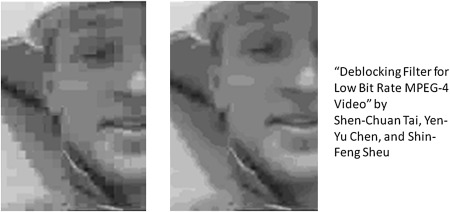
\includegraphics[width=\textwidth]{AVC_artifacts}}
\end{center}
